\section{Prior Predictive Checks}
\label{sec:prior_predictive}

% Outline:
% - State the question: what range of observables does the model produce before seeing data?
% - Describe the baseline prior ranges for eta_M, eta_M,cold, and eta_E.
% - Show the valid/failure fraction and where failures occur in parameter space.
% - Present distributions of column scale, mean velocity, velocity width, and profile shape.
% - Compare the prior predictive envelope to the scale of CLASSY-like observations.
% - Use this section to motivate any narrowing of priors before synthetic recovery.
% - End with a clear decision: whether the baseline prior is scientifically useful enough for input recovery.

\begin{figure*}[t]
\centering
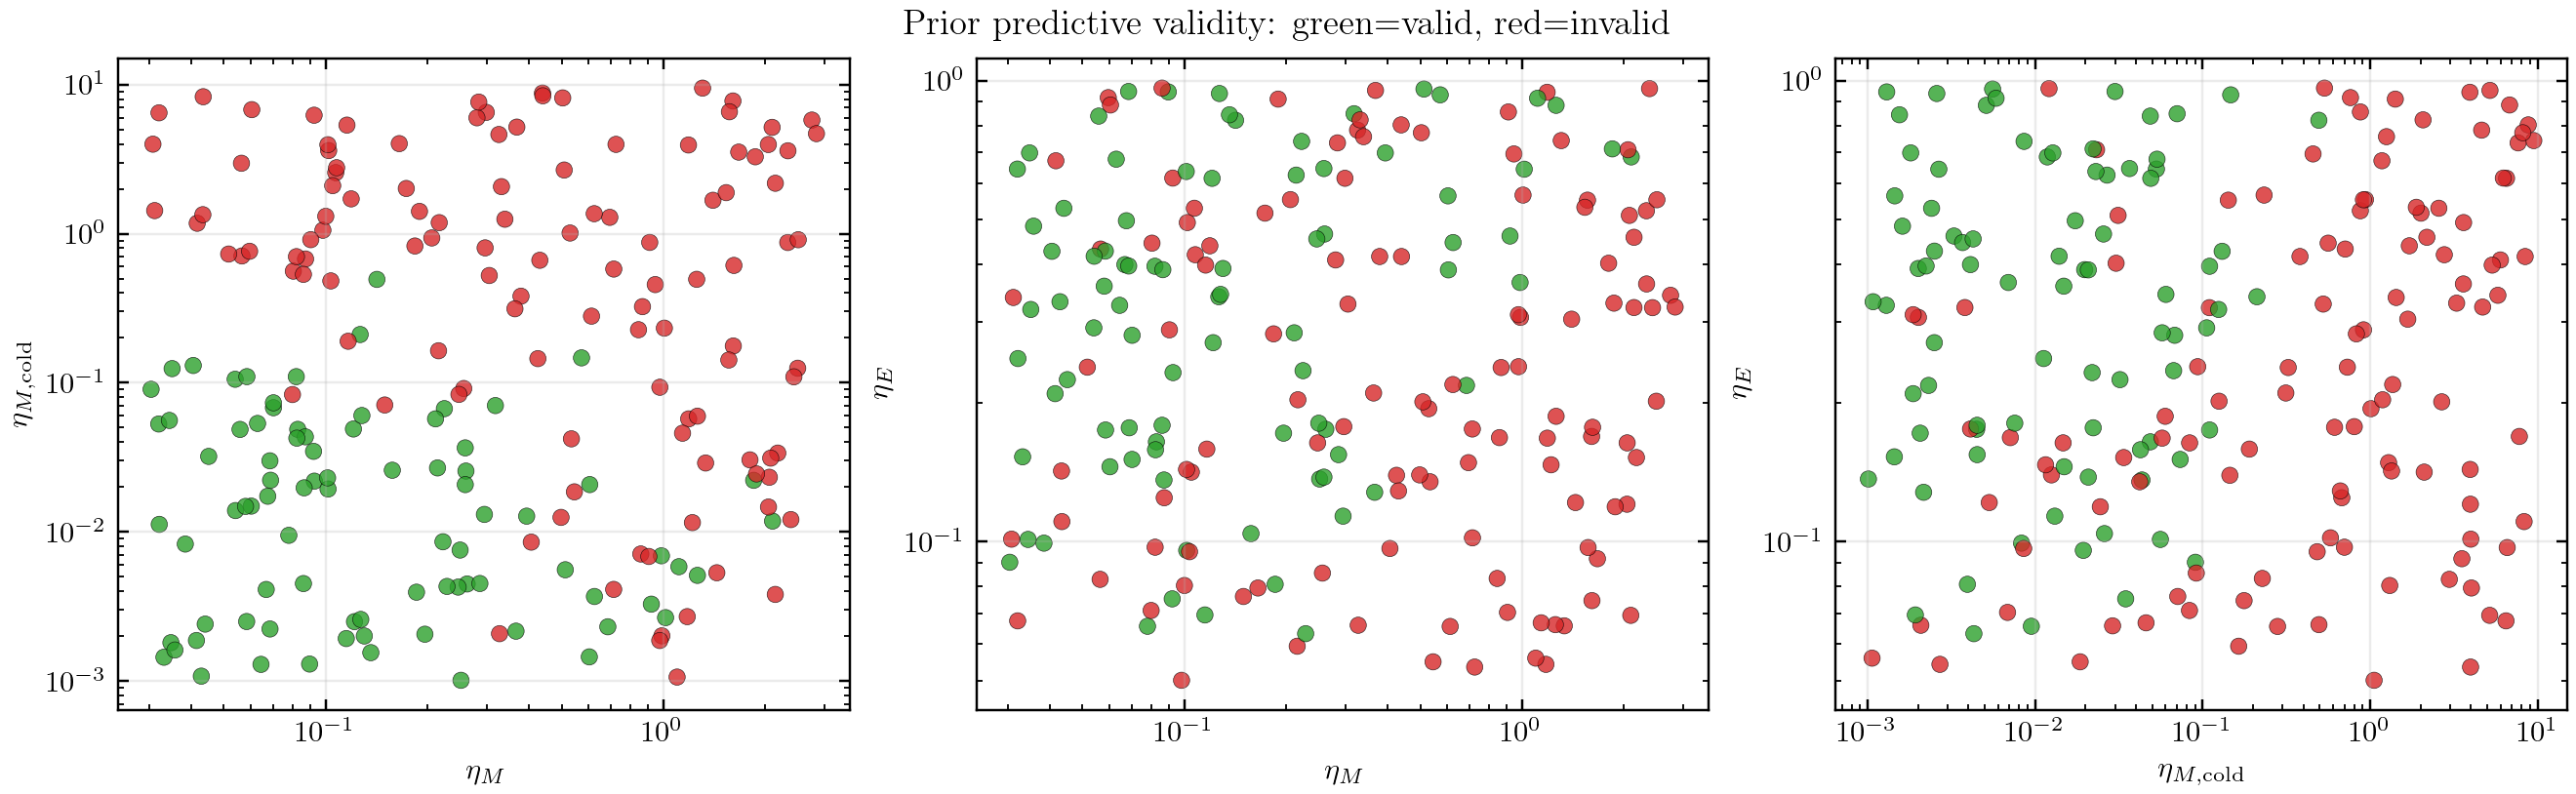
\includegraphics[width=\textwidth]{figures/prior_predictive_validity.png}
\caption{
Preliminary prior predictive validity map for the baseline three-parameter inference model.
The samples are drawn from broad exploratory priors on the hot mass loading, cold mass loading, and hot energy loading.
Green points mark parameter combinations that produce finite, physically valid observables, while red points mark failed integrations or invalid observable vectors.
This figure is meant to identify where the prior places probability on physically useful winds before any comparison with data.
}
\label{fig:prior_predictive_validity}
\end{figure*}

\begin{figure*}[t]
\centering
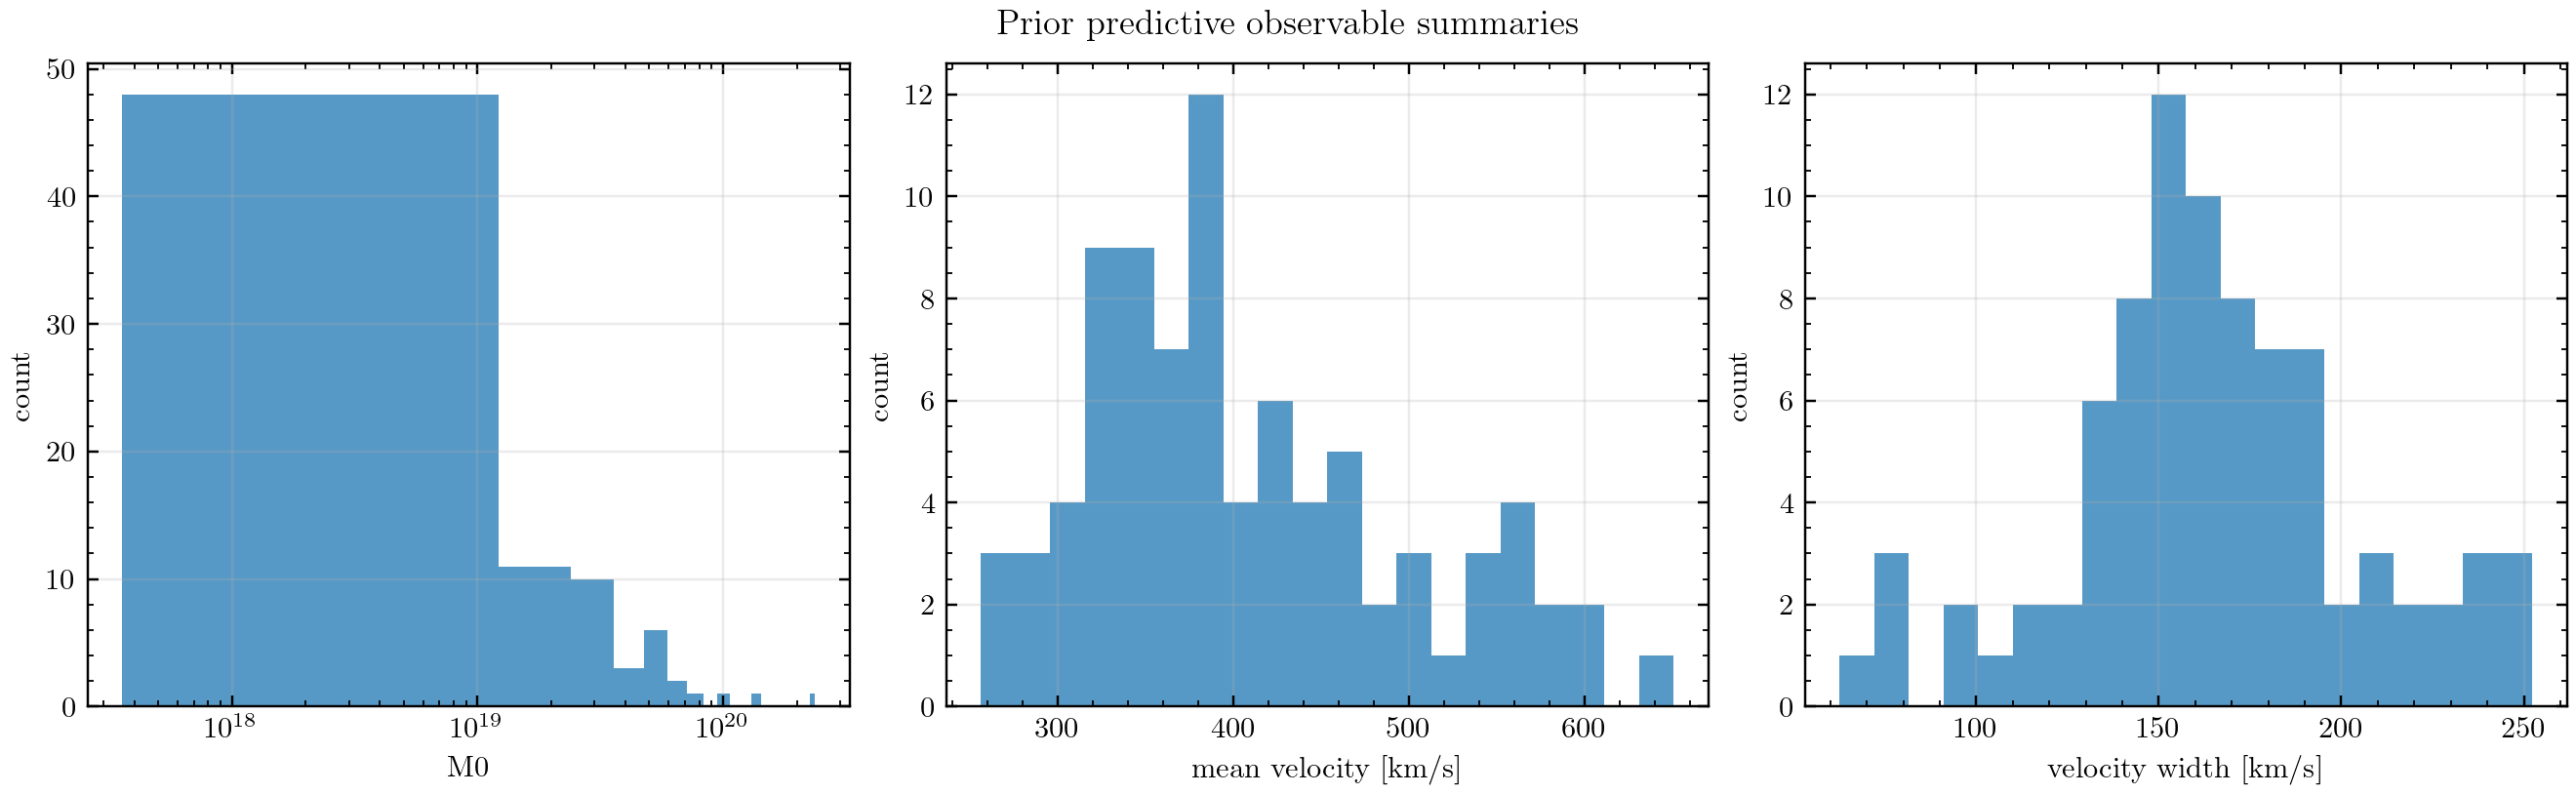
\includegraphics[width=\textwidth]{figures/prior_predictive_observable_histograms.png}
\caption{
Preliminary prior predictive distributions for three compact observable summaries computed from valid baseline samples.
The panels show the total column scale, mean velocity, and velocity width implied by the broad exploratory prior.
These distributions define the range of cool-phase absorption signatures that the current model expects before seeing the data, and therefore set the scale for the synthetic recovery tests that follow.
}
\label{fig:prior_predictive_observable_histograms}
\end{figure*}

\begin{figure*}[t]
\centering
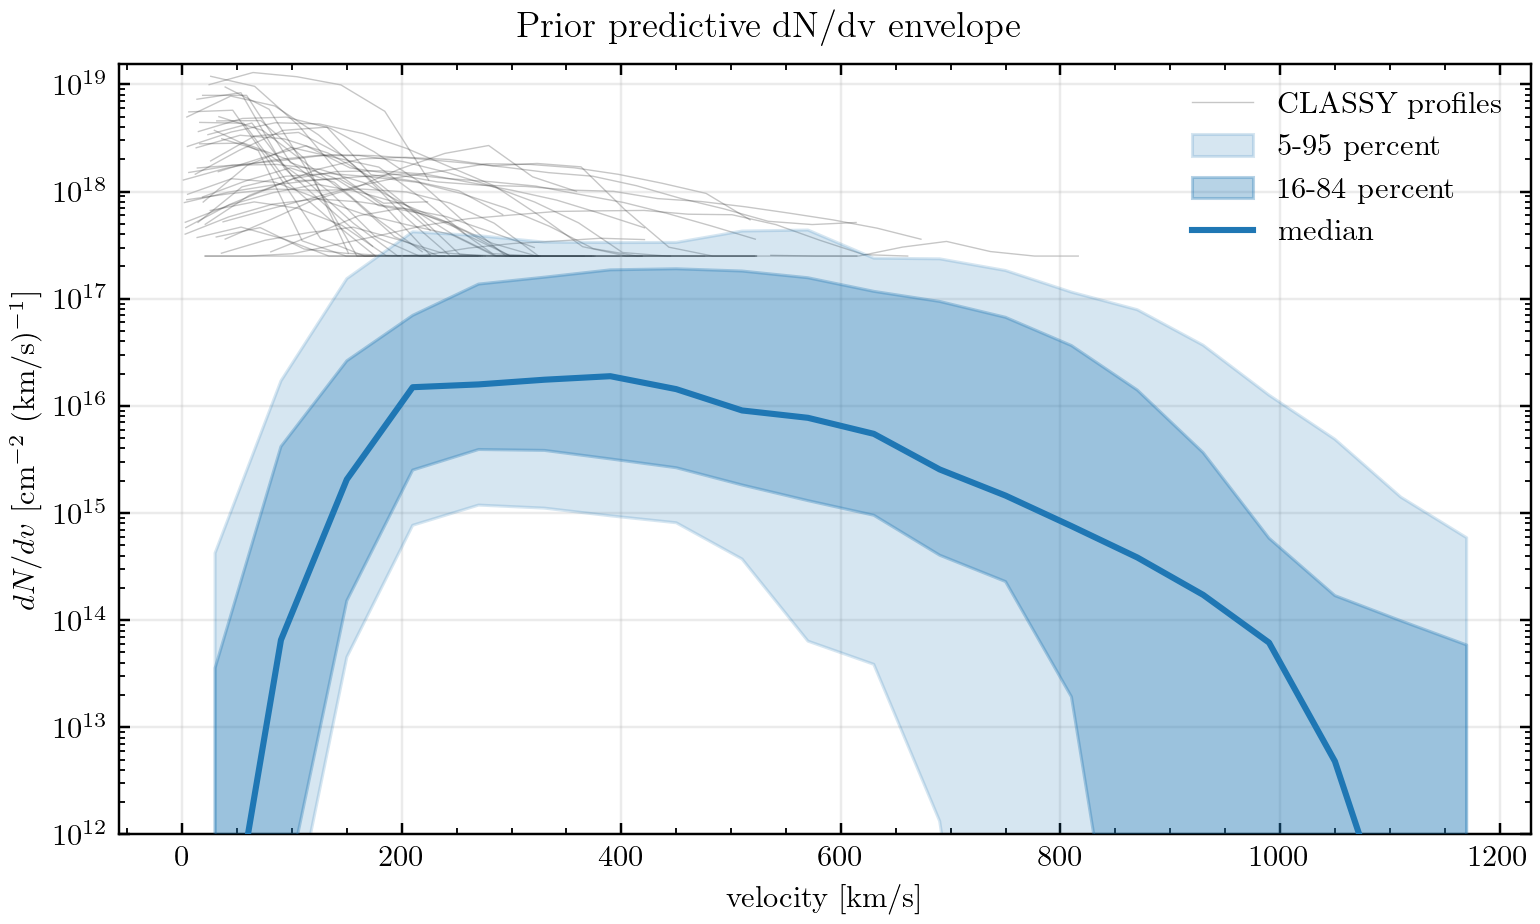
\includegraphics[width=0.82\textwidth]{figures/prior_predictive_dndv_envelope.png}
\caption{
Preliminary prior predictive envelope for the binned column-density velocity profile.
Thin gray curves show the processed CLASSY profiles after mapping blueshifted velocities to positive outflow speeds.
The shaded regions show the central prior-predictive spread among valid samples, and the solid blue curve shows the median model profile.
This comparison is intentionally imperfect: the blue prior predictive distribution is evaluated for one fixed fiducial galaxy with $\mathrm{SFR}=20\,M_\odot\,\mathrm{yr}^{-1}$, $r_\star=0.3\,\mathrm{kpc}$, and $v_{\rm circ}=150\,\mathrm{km}\,\mathrm{s}^{-1}$, while the gray curves span the full CLASSY sample with different galaxy properties.
The apparent vertical offset should therefore be read as a warning about this non-conditioned prior check, not as evidence that the model cannot fit individual CLASSY profiles.
The lower plotting limit is set to $10^{12}\,\mathrm{cm}^{-2}\,(\mathrm{km}\,\mathrm{s}^{-1})^{-1}$ to show the low-column prior tails without extending to the numerical floor used for model bookkeeping.
This profile-level check complements the moment-based summaries in Figure~\ref{fig:prior_predictive_observable_histograms} by asking whether the prior generates plausible velocity structure rather than only plausible low-order moments.
}
\label{fig:prior_predictive_dndv_envelope}
\end{figure*}
